\documentclass[12pt]{ctexart}

\usepackage[a4paper,margin=2.5cm]{geometry}
\usepackage{setspace}
\usepackage{titlesec}
\usepackage{xcolor}
\usepackage{indentfirst}
\usepackage{float}
\usepackage{graphicx}
\usepackage{float}
\usepackage{tikz}
\usetikzlibrary{arrows.meta,positioning}
\usepackage{graphicx}

\usepackage{listings}
\usepackage{xcolor}

\lstset{
    language=C++,
    basicstyle=\ttfamily\small,
    keywordstyle=\color{blue},
    stringstyle=\color{red},
    commentstyle=\color{green!50!black},
    numbers=left,
    numberstyle=\tiny,
    stepnumber=1,
    numbersep=8pt,
    breaklines=true,
    frame=single,
    tabsize=4,
    showstringspaces=false
}
\usetikzlibrary{arrows.meta}
\usetikzlibrary{arrows.meta,positioning}

\setlength{\parindent}{0em}
\setstretch{1.5}

% 标题格式
\titleformat{\section}{\bfseries\zihao{4}}{}{0em}{}
\titleformat{\subsection}{\bfseries\zihao{-4}}{}{0em}{}

% 自定义空行
\newcommand{\blankline}{\vspace{1.5em}}

\begin{document}

\begin{figure}[H]
    \centering
    
\includegraphics[width=0.70\textwidth]{img/0.png}
\end{figure}
% 首页不显示页码

\thispagestyle{empty}
\begin{center}
    {\heiti\zihao{3} 实验五}
\end{center}

{\heiti\zihao{4} 一、实验名称：}\textbf{OpenSSL综合实验}

\vspace{0.5em}

{\heiti\zihao{4} 二、实验学时：}\textbf{4学时}

\vspace{0.5em}

{\heiti\zihao{4} 三、实验内容和目的：}

本实验围绕 OpenSSL 的安装、配置、证书创建以及安全通信程序设计展开，主要包括三个部分：

\begin{enumerate}
    \item OpenSSL 源码包编译实验；
    \item 使用 OpenSSL 创建 CA，并为服务器端和客户端签发证书；
    \item 基于 OpenSSL 实现 Client/Server 安全通信程序。
\end{enumerate}

通过本实验，达到以下目的：

\begin{enumerate}
    \item 掌握 OpenSSL 源码包在 Windows 环境下的编译方法，理解其基本配置过程；
    \item 理解 CA 的作用以及数字证书的生成、签发、导出与安装流程；
    \item 熟悉 SSL/TLS 安全通信的基本原理，掌握 OpenSSL 在套接字编程中的应用方式；
    \item 学会利用 OpenSSL 提供的接口函数实现客户端与服务器之间的安全通信；
    \item 为后续修改 OpenSSL 源码、编译新版本 OpenSSL 以及开发基于 SSL 的安全程序打下基础。
\end{enumerate}

\vspace{0.5em}

{\heiti\zihao{4} 四、实验原理：}

OpenSSL 是一个开源的 SSL/TLS 协议实现软件包，支持多种操作系统平台，提供了完整的安全通信接口，能够在传统套接字编程的基础上实现机密性、完整性和身份认证等安全功能。

SSL/TLS 协议主要包括握手阶段和数据传输阶段。在握手阶段，通信双方协商协议版本、密码套件和会话密钥，并通过数字证书实现身份认证；在数据传输阶段，双方使用协商得到的密钥对应用数据进行加密和完整性保护，从而保证通信安全。

OpenSSL 与普通套接字编程紧密结合，其核心思想是在 TCP 套接字之上建立 SSL 会话。其主要过程包括：

\begin{enumerate}
    \item 创建 SSL 会话环境，即通过 \verb|SSL_CTX_new()| 申请会话上下文；
    \item 为会话环境加载证书和私钥，并通过 \verb|SSL_CTX_check_private_key()| 验证二者是否匹配；
    \item 创建 SSL 套接字，即通过 \verb|SSL_new()| 建立 SSL 结构，并通过 \verb|SSL_set_fd()| 将其与普通 TCP 套接字绑定；
    \item 客户端调用 \verb|SSL_connect()|、服务器调用 \verb|SSL_accept()| 完成 SSL 握手；
    \item 握手完成后，双方通过 \verb|SSL_read()| 和 \verb|SSL_write()| 完成加密数据传输；
    \item 通信结束后，通过 \verb|SSL_shutdown()|、\verb|SSL_free()| 和 \verb|SSL_CTX_free()| 释放相关资源。
\end{enumerate}

在证书体系中，CA（Certificate Authority，证书颁发机构）负责签发和管理数字证书。服务器证书用于证明服务器身份，客户端证书用于证明客户端身份。通过将 CA 根证书导入受信任的根证书存储区，可以使系统信任该 CA 所签发的服务器证书和客户端证书，从而建立可信的 SSL/TLS 通信关系。

\vspace{0.5em}

{\heiti\zihao{4} 五、实验器材（设备、元器件）：}

\begin{enumerate}
    \item 安装 Windows 7 的主机或宿主机环境；
    \item 安装 Windows Server 2003 的虚拟机或服务器环境；
    \item Visual Studio 2010 编程环境；
    \item ActivePerl 5.20.1.2000 及以上版本；
    \item OpenSSL 0.9.8zc 源码包；
    \item 编译生成的 OpenSSL 可执行程序、头文件及库文件；
    \item IIS 服务环境；
    \item 浏览器及证书管理工具。
\end{enumerate}

\vspace{0.5em}

{\heiti\zihao{4} 六、实验步骤：}






{\heiti\zihao{4} 七、实验数据及结果分析：}

\textbf{（1）OpenSSL源码编译与安装结果分析}

\begin{figure}[htbp]
    \centering
    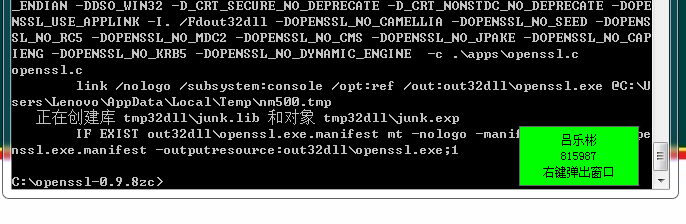
\includegraphics[width=0.48\textwidth]{img/2045fd4d02a0f7aa3c0f9e8f73ea1cf1.png}
    \hfill
    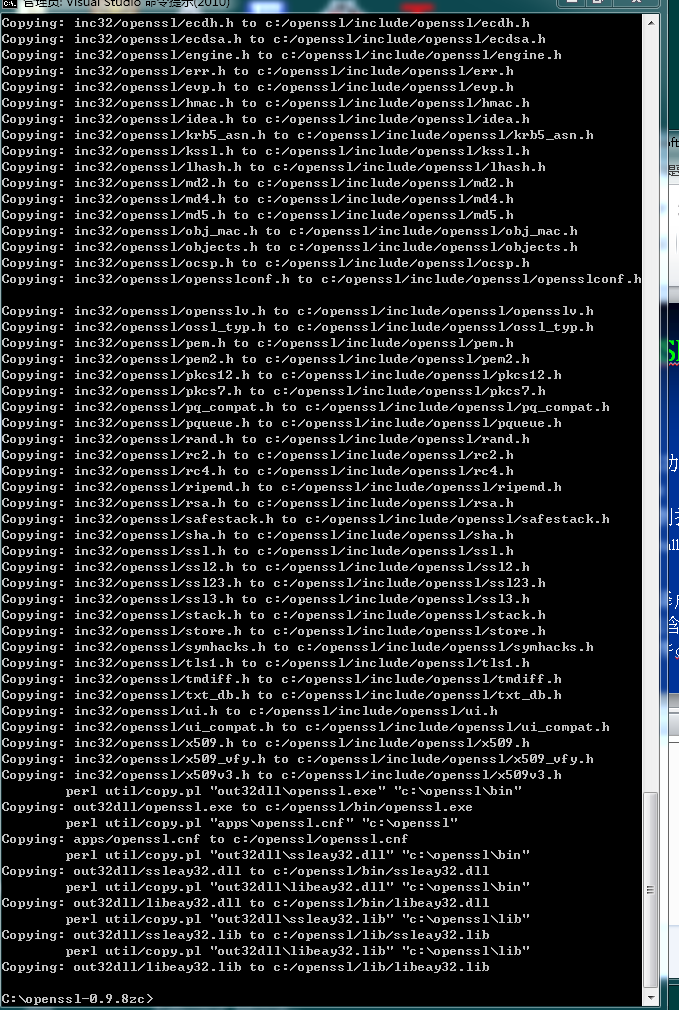
\includegraphics[width=0.48\textwidth]{img/ae5f2b851e9f1664631ffe6f473fdc15.png}
    \caption{OpenSSL源码编译与安装过程}
\end{figure}

从图中可以看出，实验首先在 Windows 环境下完成了 OpenSSL 源码的编译与安装。编译过程中成功生成了可执行程序、动态链接库及相关目标文件；安装过程中，系统将头文件、库文件和配置文件复制到指定目录中。该结果说明 OpenSSL 源码已经能够在当前实验环境下被正确编译和部署，为后续 CA 创建、证书签发以及 SSL 安全通信程序开发提供了基础运行环境。

\begin{figure}[htbp]
    \centering
    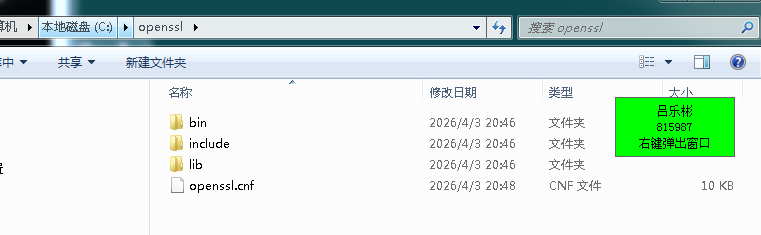
\includegraphics[width=0.62\textwidth]{img/058c4ae139be9a07dac514818b3fd5f1.png}
    \caption{OpenSSL安装完成后的目录结构}
\end{figure}

由安装完成后的目录结构可见，\texttt{C:\textbackslash openssl} 目录下已经生成了 \texttt{bin}、\texttt{include}、\texttt{lib} 以及 \texttt{openssl.cnf} 等关键文件。其中，\texttt{bin} 目录用于存放 OpenSSL 可执行文件及相关动态链接库，\texttt{include} 目录用于存放头文件，\texttt{lib} 目录用于存放库文件，\texttt{openssl.cnf} 则用于后续证书生成和签发时的配置。该结果说明 OpenSSL 安装成功。

\textbf{（2）CA工作目录及基础文件创建结果分析}

\begin{figure}[htbp]
    \centering
    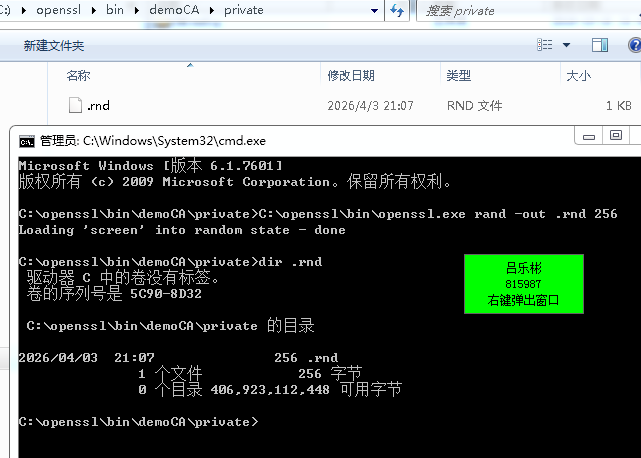
\includegraphics[width=0.48\textwidth]{img/a21b4e20e9f8ea2838b6d8a7c34e7c1b.png}
    \hfill
    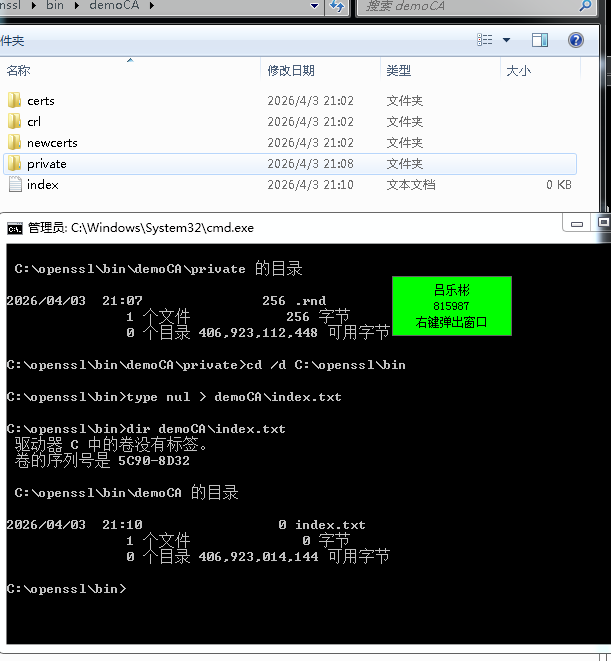
\includegraphics[width=0.48\textwidth]{img/9ad684cd923b1d3fa2db7de4978c6f9d.png}
    \caption{随机数文件（利用openssl指令生成）与文本数据库文件创建结果}
\end{figure}

在创建 CA 之前，需要首先建立 OpenSSL 所要求的目录树及辅助文件。实验中先在 \texttt{demoCA\textbackslash private} 目录下生成了随机数文件 \texttt{.rnd}，该文件用于为后续密钥生成过程提供随机性来源。随后在 \texttt{demoCA} 目录下创建了空的文本数据库文件 \texttt{index.txt}，用于记录后续签发证书的相关信息。这两个文件的建立说明 CA 工作环境已开始初始化。

\begin{figure}[htbp]
    \centering
    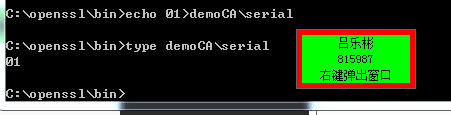
\includegraphics[width=0.50\textwidth]{img/f85bb3f6461513c2d48576157315a78f.png}
    \caption{证书序列号文件serial创建结果}
\end{figure}

实验中还创建了证书序列号文件 \texttt{serial}，并写入初始值 \texttt{01}。该文件用于控制 CA 所签发证书的编号顺序，是后续服务器证书和客户端证书签发过程中必不可少的组成部分。该步骤完成后，说明 CA 的基础数据库环境已搭建完毕。

\textbf{（3）根证书生成结果分析}

\begin{figure}[htbp]
    \centering
    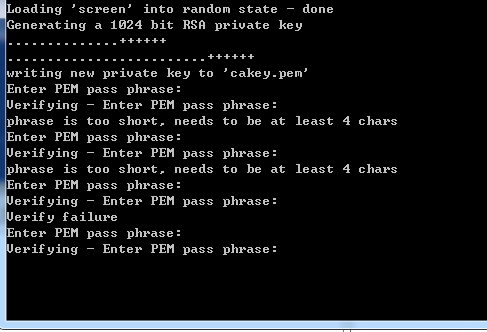
\includegraphics[width=0.48\textwidth]{img/5f68899e87d2d8336558e913bf76331d.png}
    \hfill
    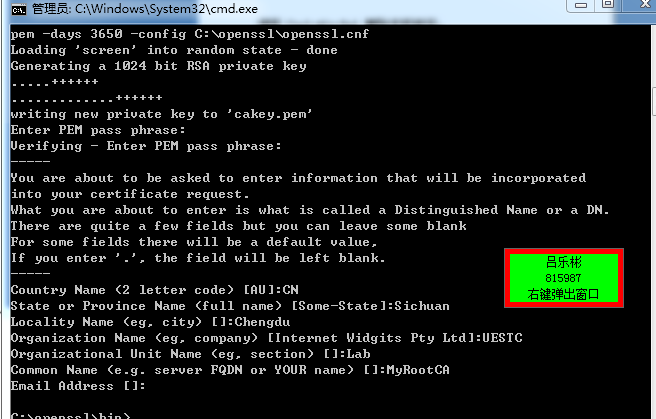
\includegraphics[width=0.48\textwidth]{img/45cc44336c925632baba0415fdd3e071.png}
    \caption{CA私钥与根证书生成过程}
\end{figure}

在生成根证书的过程中，首先生成了 CA 私钥文件，并设置了私钥口令。从截图中可以看出，实验过程中曾出现口令长度不足的提示，随后重新输入符合要求的口令后继续执行。这说明 OpenSSL 在私钥保护上具有基本的安全限制。之后，按照配置文件要求填写国家、省份、城市、组织、组织单位及公共名称等信息，最终成功生成了自签名根证书。

\begin{figure}[htbp]
    \centering
    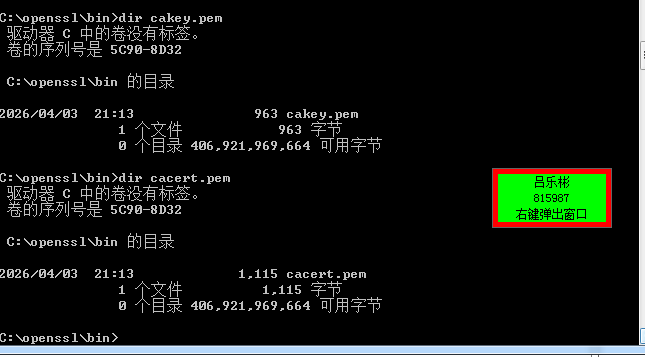
\includegraphics[width=0.48\textwidth]{img/88fc139f2501b5595d8689cc7cddd6c8.png}
    \hfill
    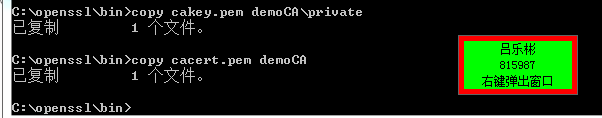
\includegraphics[width=0.48\textwidth]{img/6eb730ef08e46636fb96157226ad2851.png}
    \caption{根私钥与根证书生成并复制到demoCA目录}
\end{figure}

由图中可见，根私钥文件 \texttt{cakey.pem} 和根证书文件 \texttt{cacert.pem} 已成功生成。随后将 \texttt{cakey.pem} 复制到 \texttt{demoCA\textbackslash private} 目录中，并将 \texttt{cacert.pem} 复制到 \texttt{demoCA} 目录中，满足了 OpenSSL CA 工作目录的要求。这说明 CA 的根信任基础已经建立完成。

\textbf{（4）服务器证书签发与查看结果分析}

\begin{figure}[htbp]
    \centering
    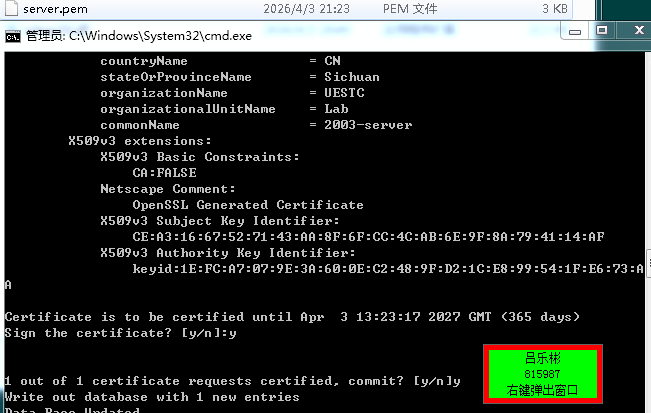
\includegraphics[width=0.48\textwidth]{img/7d712858d1454615d31be0e8fd5d7518.png}
    \hfill
    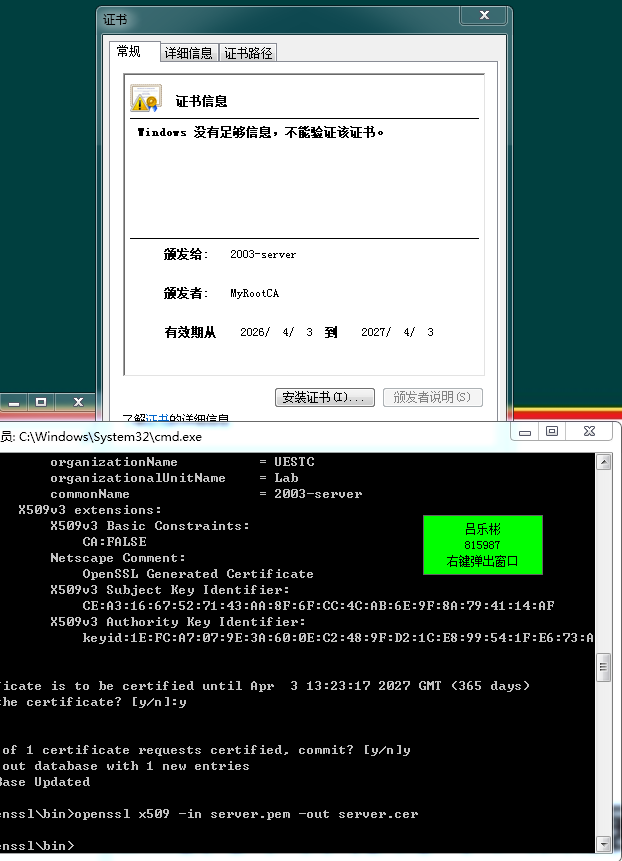
\includegraphics[width=0.48\textwidth]{img/147492c06a7373e02cacc4b0e70fac49.png}
    \caption{服务器证书签发及格式转换结果}
\end{figure}

在服务器证书生成阶段，首先利用 CA 对服务器证书请求文件进行签名，得到服务器证书 \texttt{server.pem}。从图中可以看到，证书中已经包含国家、省份、组织、组织单位和公共名称等字段，同时具备 X509v3 的相关扩展信息，说明服务器证书已被成功签发。之后再通过格式转换命令将 \texttt{server.pem} 转换为 IIS 可导入的 \texttt{server.cer} 文件，为后续网站绑定证书做好准备。

\begin{figure}[htbp]
    \centering
    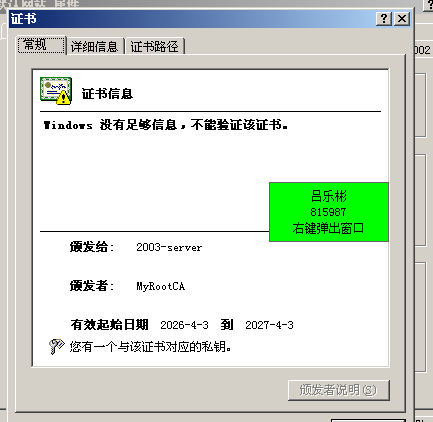
\includegraphics[width=0.48\textwidth]{img/72721bfaee9fe9d32c09b1b790a58eb4.png}
    \hfill
    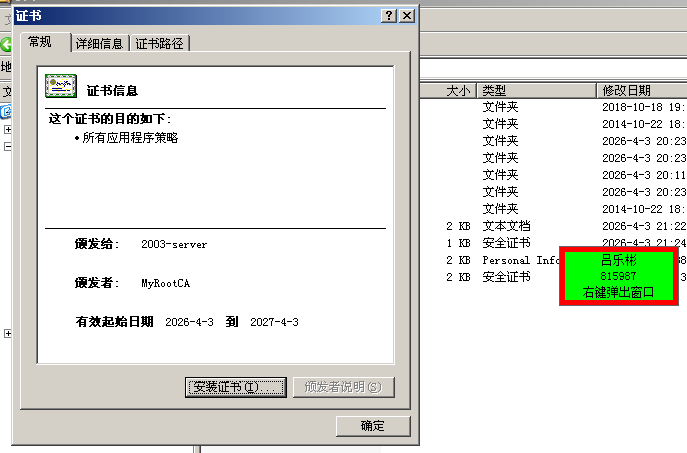
\includegraphics[width=0.48\textwidth]{img/a7af3283280d8e6690536004b906d47d.png}
    \caption{服务器证书查看结果}
\end{figure}

从服务器证书查看界面可以看到，证书已经能够正常显示颁发给对象、颁发者及有效期等信息，说明服务器证书文件本身生成成功。其中，前一截图反映的是服务器证书生成后的中间查看结果，此时系统尚未完全建立信任链，因此验证信息仍不完整；后一截图则表明服务器证书已经能够被正常安装和查看，为 IIS 绑定 SSL 证书提供了前提条件。

\textbf{（5）客户端证书生成与导出结果分析}

\begin{figure}[htbp]
    \centering
    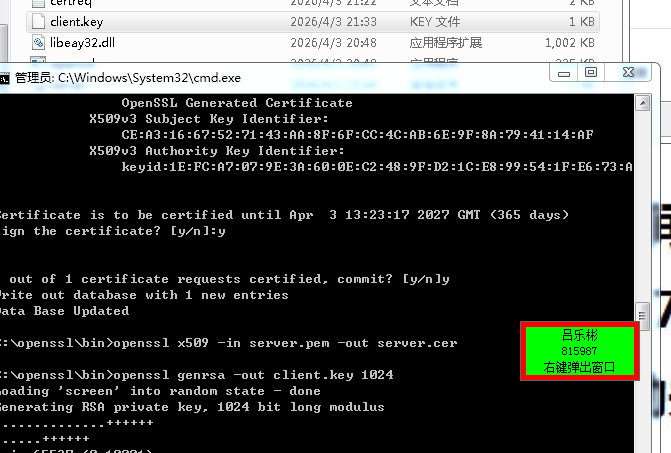
\includegraphics[width=0.48\textwidth]{img/7971be5d96a28339f9cac78d849a7103.png}
    \hfill
    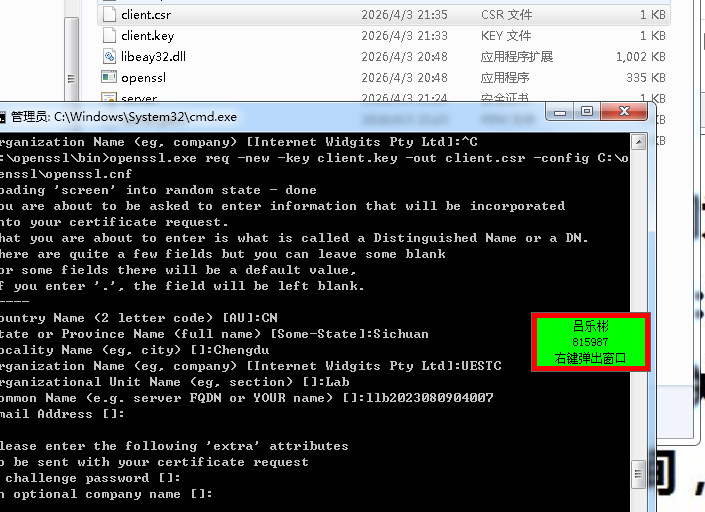
\includegraphics[width=0.48\textwidth]{img/5817532d33e019e6b31be8922e35ab87.png}
    \caption{客户端密钥生成与证书请求信息填写}
\end{figure}

在客户端证书生成阶段，首先利用 \texttt{genrsa} 命令生成客户端私钥 \texttt{client.key}，随后使用该私钥生成证书请求文件 \texttt{client.csr}。从截图中可以看出，实验过程中填写了国家、省份、城市、组织、组织单位以及公共名称等证书主题信息。这说明客户端证书请求文件已按要求生成，为后续 CA 签发客户端证书奠定了基础。

\begin{figure}[htbp]
    \centering
    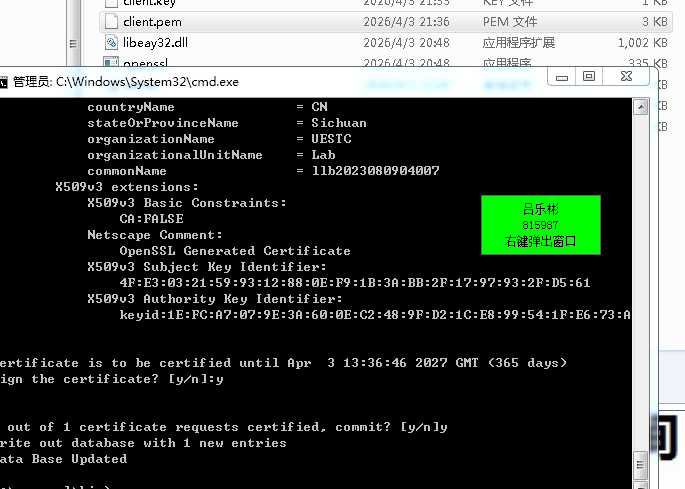
\includegraphics[width=0.48\textwidth]{img/d1a1a067aeca88c9b8654045ac709f5f.png}
    \hfill
    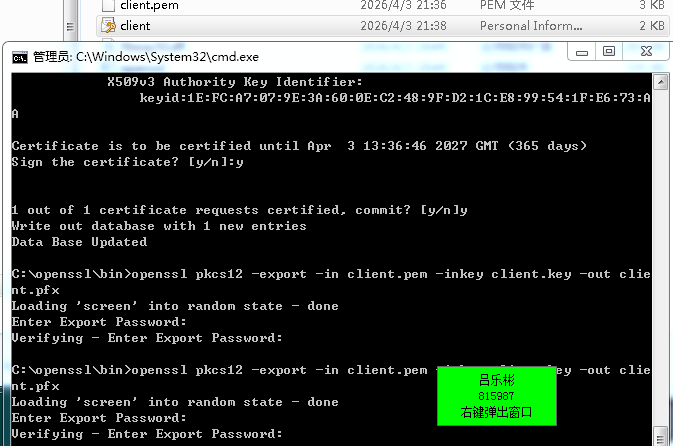
\includegraphics[width=0.48\textwidth]{img/6161179c902f9fe631e91c41ffa45d6f.png}
    \caption{客户端证书签发与PFX格式导出结果}
\end{figure}

由图中可见，CA 已成功对客户端证书请求进行签发，生成了客户端证书文件 \texttt{client.pem}。随后通过 \texttt{pkcs12} 命令将客户端证书和私钥进一步封装为 \texttt{client.pfx} 文件，以便在浏览器或操作系统证书管理器中导入使用。该结果说明客户端证书已经准备完成，后续只需导入即可参与双向认证。

\textbf{（6）客户端证书导入与查看结果分析}

\begin{figure}[htbp]
    \centering
    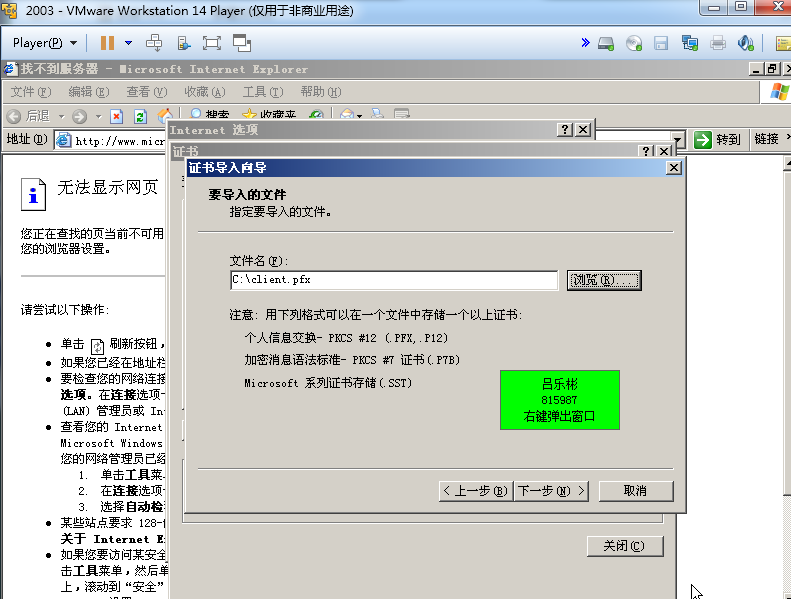
\includegraphics[width=0.48\textwidth]{img/b1f31a8b264bd8f9e74772cd7d007084.png}
    \hfill
    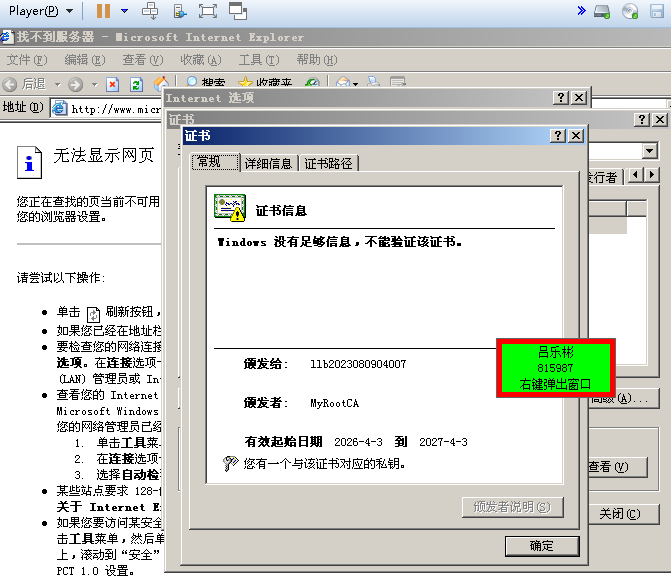
\includegraphics[width=0.48\textwidth]{img/fc1975b09a431f640011e2aea8e7b15f.png}
    \caption{客户端证书导入与初步查看结果}
\end{figure}

在客户端证书使用阶段，首先通过证书导入向导选择 \texttt{client.pfx} 文件进行导入。导入后可以查看到客户端证书的基本信息，包括颁发给对象、颁发者及有效期等内容，并且界面显示“您有一个与该证书对应的私钥”，说明客户端私钥与证书已经正确关联。不过，从初步查看界面仍可见系统尚未完全验证该证书，这说明此时还需要进一步完成根证书的信任安装。

\begin{figure}[htbp]
    \centering
    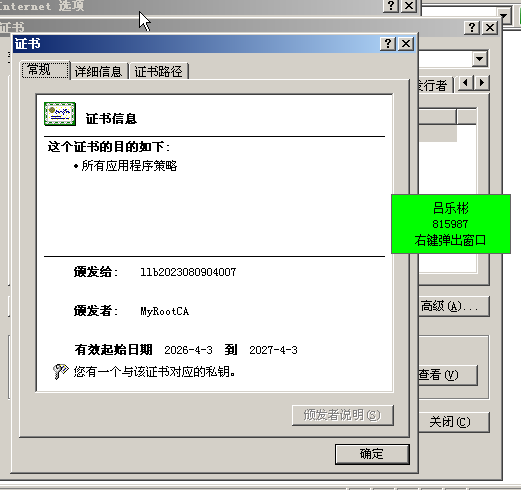
\includegraphics[width=0.62\textwidth]{img/d06fd0083a5ebc348f194474ccbaacb0.png}
    \caption{客户端证书导入后的查看结果}
\end{figure}

继续查看客户端证书可以发现，证书已经能够以正常形式显示其用途、颁发者和有效期等信息，且对应私钥存在。这表明客户端证书已经成功导入到系统中，具备了后续访问启用客户端证书认证网站的条件。

\textbf{（7）根证书安装与信任关系结果分析}

\begin{figure}[htbp]
    \centering
    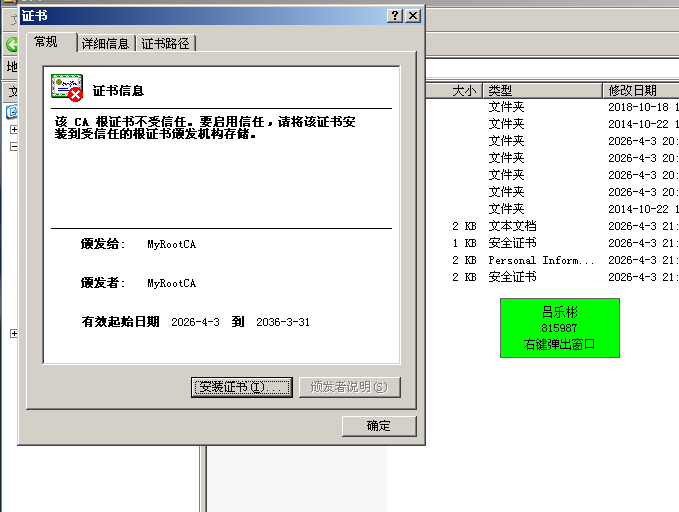
\includegraphics[width=0.48\textwidth]{img/272c9b3cae1e381629c6978d302af53d.png}
    \hfill
    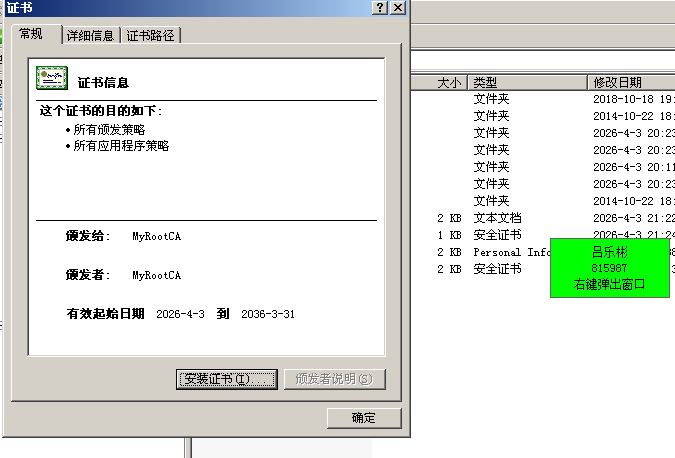
\includegraphics[width=0.48\textwidth]{img/9850ed80a82e1813c02219e9138cc3e6.png}
    \caption{根证书查看与安装前后状态}
\end{figure}

在根证书安装阶段，首先查看根证书信息时，系统提示“该 CA 根证书不受信任。要启用信任，请将该证书安装到受信任的根证书颁发机构存储区”，说明此时操作系统尚未建立对该自签名根证书的信任关系。随后对根证书进行安装并再次查看后，可以正常显示根证书的颁发给对象、颁发者及有效期等信息。该过程表明，实验已经完成了根证书导入操作，为后续服务器证书和客户端证书通过信任链验证创造了条件。

\textbf{（8）IIS站点SSL安全配置结果分析}

\begin{figure}[htbp]
    \centering
    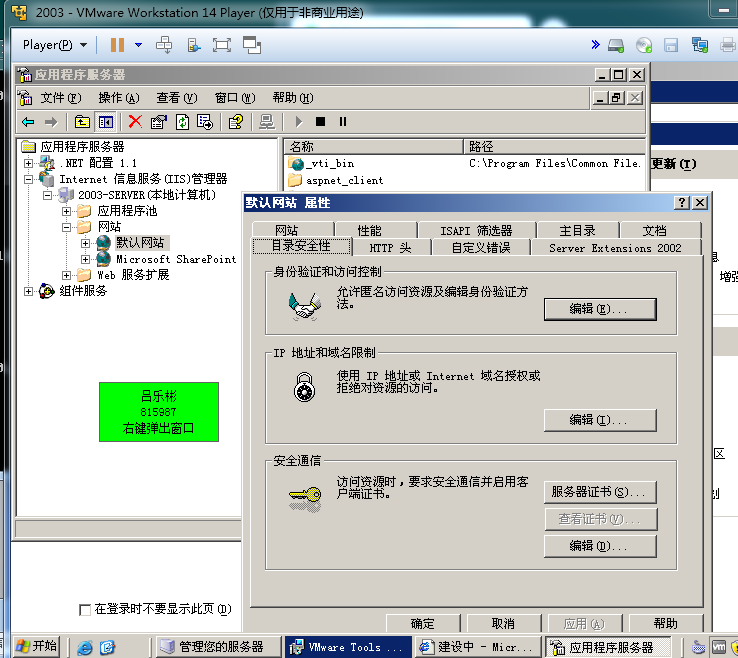
\includegraphics[width=0.48\textwidth]{img/b9432b40e59c9d31a375a3ff33986176.png}
    \hfill
    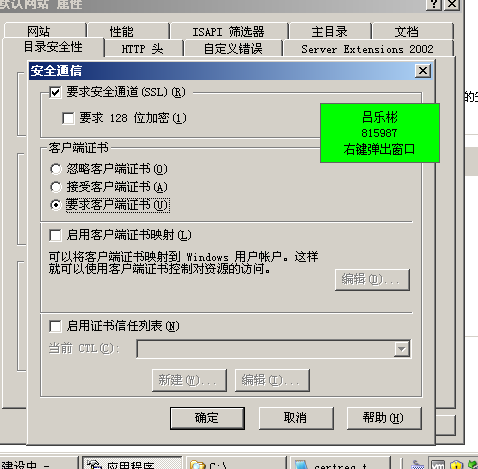
\includegraphics[width=0.48\textwidth]{img/2ba1c8d8a7da0f7c5222d5f4f9ea53bd.png}
    \caption{IIS默认网站SSL安全设置结果}
\end{figure}

在 IIS 配置阶段，实验进入默认网站的目录安全属性页，并进一步设置 SSL 安全通信参数。从图中可以看到，站点已勾选“要求安全通道（SSL）”，同时在客户端证书选项中选择了“要求客户端证书”。这表明服务器端已经按照实验要求启用了 SSL 双向认证机制，即客户端在访问网站时不仅要通过 HTTPS 建立安全连接，还必须提交有效的客户端证书。

\textbf{（9）IIS网站访问结果分析}

\begin{figure}[htbp]
    \centering
    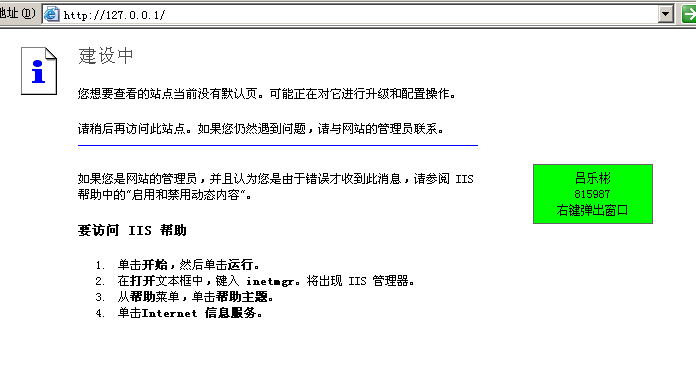
\includegraphics[width=0.48\textwidth]{img/d13291102254ef3933bfa92e938b8500.png}
    \hfill
    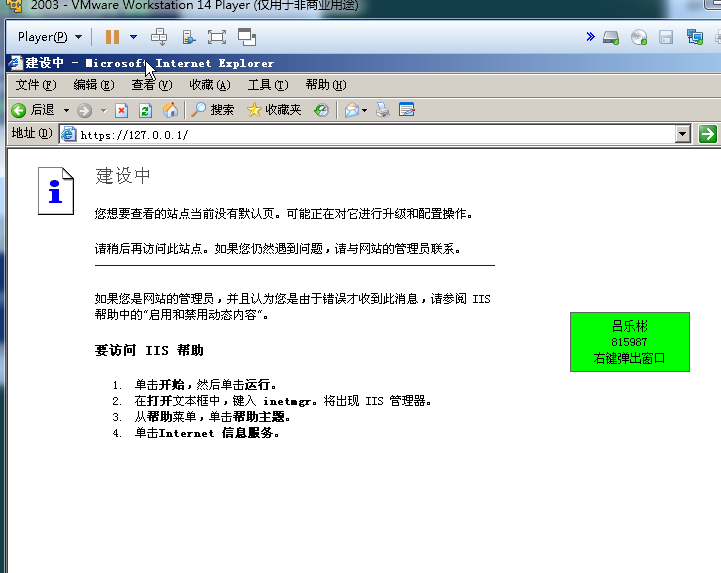
\includegraphics[width=0.48\textwidth]{img/cb9b82b2f55cea023f0b77629638ab08.png}
    \caption{IIS网站HTTP与HTTPS访问结果}
\end{figure}

从访问结果可以看出，浏览器首先能够正常打开默认网站页面，说明 IIS 服务已经成功启动，服务器端 Web 服务环境可正常响应浏览器请求。进一步访问 \texttt{https://127.0.0.1/} 后，页面同样能够正常显示，这说明服务器证书绑定、SSL 配置以及客户端证书认证流程已经基本生效。也就是说，实验已经完成了从普通 Web 服务到 HTTPS 安全访问的验证过程。





\textbf{（10）基于OpenSSL实现C/S程序(代码见附录1)}

在完成 OpenSSL 的编译安装以及证书创建实验之后，进一步基于 OpenSSL 编写客户端与服务器端程序，以验证 OpenSSL 在 C/S 安全通信中的实际应用效果。本实验中，服务器端加载服务器证书和私钥，客户端加载受信任证书，对服务器证书进行校验，并通过本地回环地址 \texttt{127.0.0.1} 建立 SSL 安全连接。

实现过程中，首先分别编写服务器端和客户端程序。在服务器端，先初始化 OpenSSL 环境，创建 SSL 会话上下文，并加载服务器证书和私钥；随后创建 TCP 监听套接字，在接收到客户端连接后，通过 \texttt{SSL\_accept()} 完成 SSL 握手。客户端则在初始化 OpenSSL 环境后，加载 CA 证书，并设置对服务器证书进行验证；建立 TCP 连接后，通过 \texttt{SSL\_connect()} 发起握手，并在握手完成后利用 \texttt{SSL\_get\_verify\_result()} 检查服务器证书是否合法。握手和校验均通过后，客户端向服务器发送测试消息，服务器接收后返回响应内容，从而完成一次基于 SSL 的安全通信。

程序的主要实现要点如下：

\begin{verbatim}
SSL_CTX* ctx = SSL_CTX_new(SSLv23_server_method());
SSL_CTX_use_certificate_file(ctx, "server.crt", SSL_FILETYPE_PEM);
SSL_CTX_use_PrivateKey_file(ctx, "server.key", SSL_FILETYPE_PEM);
\end{verbatim}

上述代码用于服务器端创建 SSL 上下文并加载服务器证书与私钥。

\begin{verbatim}
SSL_CTX* ctx = SSL_CTX_new(SSLv23_client_method());
SSL_CTX_load_verify_locations(ctx, "ca.crt", nullptr);
SSL_CTX_set_verify(ctx, SSL_VERIFY_PEER, nullptr);
\end{verbatim}

上述代码用于客户端加载受信任证书并启用服务器证书校验。

\begin{verbatim}
SSL_accept(ssl);   // 服务器端完成SSL握手
SSL_connect(ssl);  // 客户端发起并完成SSL握手
\end{verbatim}

上述代码表明客户端与服务器并非进行普通 TCP 通信，而是完成了基于 SSL/TLS 的安全握手。

\begin{verbatim}
long result = SSL_get_verify_result(ssl);
if (result == X509_V_OK) {
    // 证书校验成功
}
\end{verbatim}

该部分用于客户端验证服务器证书是否通过校验，是本实验要求的关键环节之一。

\begin{verbatim}
SSL_write(ssl, msg, strlen(msg));
SSL_read(ssl, buf, sizeof(buf) - 1);
\end{verbatim}

上述代码用于在 SSL 握手完成后实现客户端与服务器之间的安全数据传输。

\begin{figure}[htbp]
    \centering
    
\includegraphics[width=0.88\textwidth]{img/1.png}
    \caption{OpenSSL客户端与服务器完成SSL握手、证书校验及安全通信}
\end{figure}

从图中可以看出，服务器端首先成功进入监听状态，显示 \texttt{[Server] listening on 127.0.0.1:4433}，说明服务器已经正确完成套接字创建、绑定与监听。随后客户端成功建立 TCP 连接，并完成 SSL 握手，客户端与服务器两侧均输出了 \texttt{SSL handshake success}，表明 SSL/TLS 握手过程已经正常完成。

进一步地，客户端输出了 \texttt{Certificate verify success}，同时还打印了服务器证书的主题信息和签发者信息，说明客户端已经成功完成了对服务器证书的校验。这与实验要求“对 OpenSSL 客户端进行证书校验”完全对应，证明本实验不仅实现了客户端与服务器之间的通信，而且完成了服务器身份认证。

在握手和证书校验通过后，客户端向服务器发送了消息 \texttt{Hello from SSL client.}，服务器成功接收并输出该消息；随后服务器向客户端返回 \texttt{Hello, this is SSL server.}，客户端也正确接收到了服务器的响应。这表明客户端与服务器已经在 SSL 保护下完成了一次完整的数据交互过程，说明基于 OpenSSL 的 C/S 安全通信程序已能够正常工作。

综上所述，本部分实验成功实现了基于 OpenSSL 的客户端与服务器程序设计，完成了 SSL/TLS 握手、服务器证书校验以及安全数据收发，表明实验（3）要求已经完成。完整源代码见附录。




{\heiti\zihao{4} 八、实验结论、心得体会和改进建议：}

\textbf{1. 实验结论}

{\heiti\zihao{4} 八、实验结论：}



\textbf{查看 CA、客户端和服务器证书}

实验中分别查看了 CA 根证书、客户端证书和服务器证书的基本信息，能够看到证书的颁发者、颁发给对象、有效期等内容，并完成了相应截图。

\begin{figure}[htbp]
    \centering
    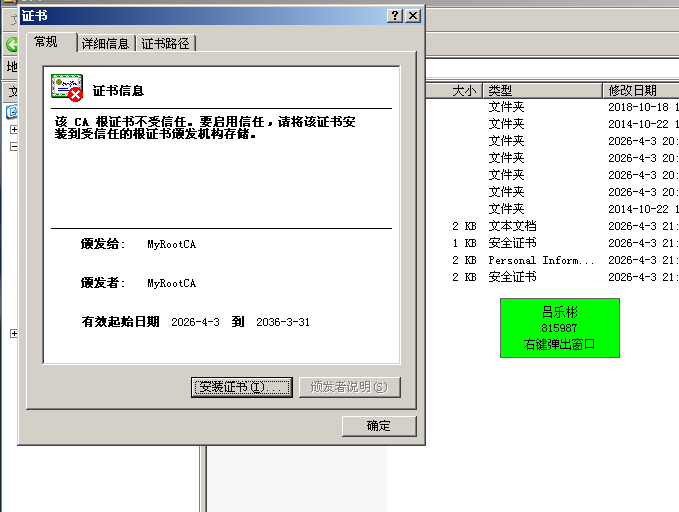
\includegraphics[width=0.32\textwidth]{img/272c9b3cae1e381629c6978d302af53d.png}
    \hfill
    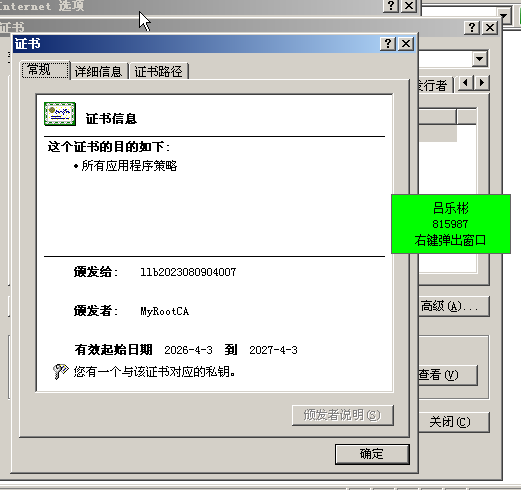
\includegraphics[width=0.32\textwidth]{img/d06fd0083a5ebc348f194474ccbaacb0.png}
    \hfill
    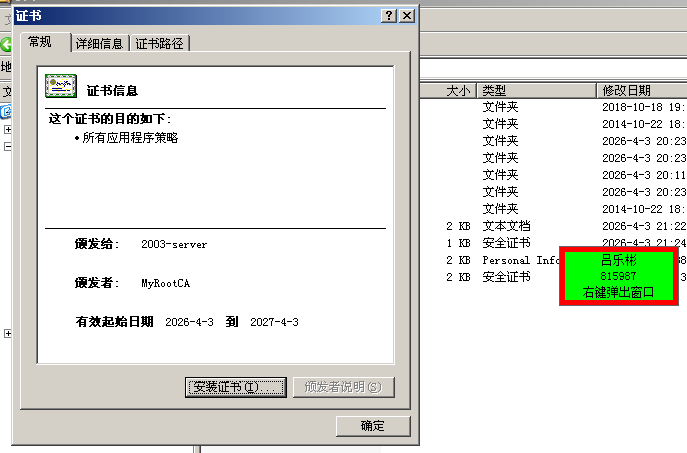
\includegraphics[width=0.32\textwidth]{img/a7af3283280d8e6690536004b906d47d.png}
    \caption{CA证书、客户端证书和服务器证书查看结果}
\end{figure}

\textbf{正确配置服务器的默认网站}

在服务器默认网站的 SSL 配置过程中，正确设置了“要求安全通道（SSL）”以及“要求客户端证书”等选项，完成了默认网站的安全属性配置，并进行了截图。

\begin{figure}[htbp]
    \centering
    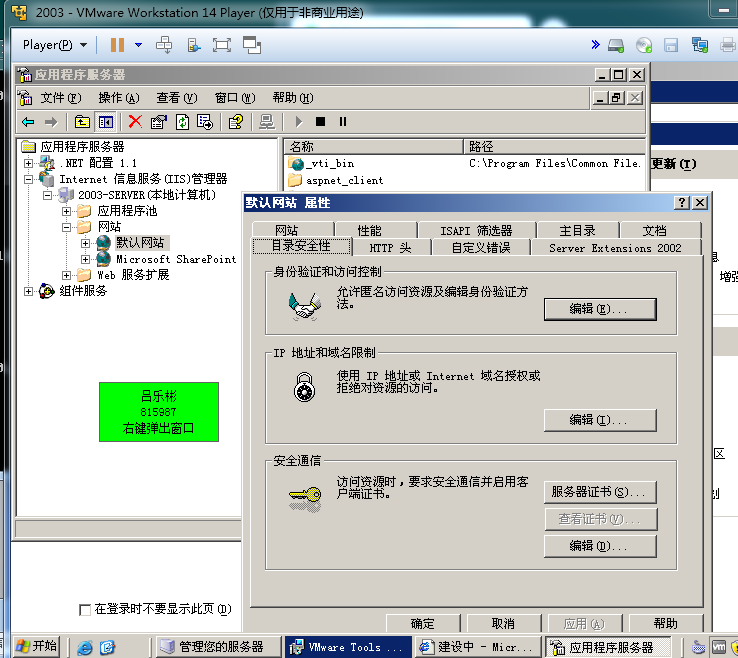
\includegraphics[width=0.48\textwidth]{img/b9432b40e59c9d31a375a3ff33986176.png}
    \hfill
    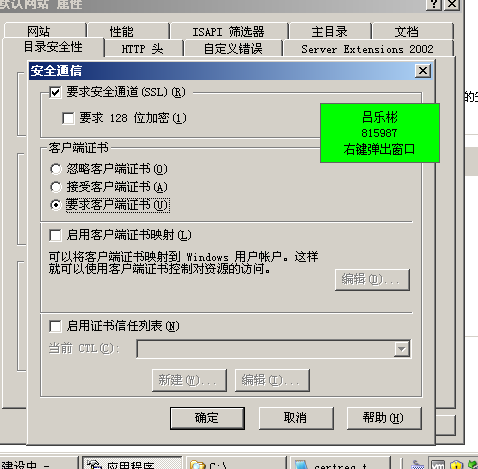
\includegraphics[width=0.48\textwidth]{img/2ba1c8d8a7da0f7c5222d5f4f9ea53bd.png}
    \caption{服务器默认网站SSL配置结果}
\end{figure}

\textbf{利用 https 成功访问默认网站}

实验最后利用 \texttt{https://127.0.0.1/} 成功访问了服务器默认网站，说明服务器证书、客户端证书及 SSL 配置已经基本生效，并完成了访问结果截图。

\begin{figure}[htbp]
    \centering
    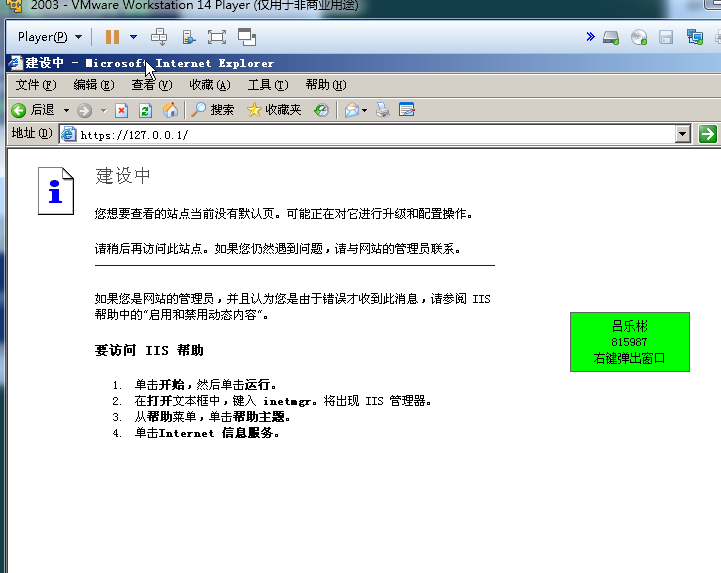
\includegraphics[width=0.68\textwidth]{img/cb9b82b2f55cea023f0b77629638ab08.png}
    \caption{通过https成功访问默认网站}
\end{figure}





\textbf{2. 心得体会}

通过本实验，我进一步理解了 SSL/TLS 协议的基本工作过程，尤其是握手协商、证书认证和加密传输等关键机制。相比仅停留在理论学习阶段，本实验将 OpenSSL 的编译、证书签发和程序开发联系起来，使我对安全通信系统的实现过程有了更加直观和深入的认识。同时，我也体会到实验中配置文件、证书字段和系统环境一致性的重要性，任何细节配置错误都可能导致实验失败，因此在实际操作中必须认真细致。

\textbf{3. 改进建议}

\begin{enumerate}
    \item 建议实验环境尽量统一，例如统一操作系统版本、开发工具和 OpenSSL 版本，以减少环境差异对实验结果的影响；
    \item 建议在实验指导中增加更多关于常见错误的排查说明，如 Perl 环境变量问题、编译错误、证书字段不匹配问题等；
    \item 建议补充对 SSL/TLS 抓包分析、证书字段解析和握手流程验证等内容，使实验结果分析更加完整；
    \item 建议在完成基础实验后，进一步扩展到更高版本 OpenSSL 或更现代的 TLS 配置实践，以增强实验的现实意义和工程价值。
\end{enumerate}

\appendix
\section*{附录：实验（3）源代码}

\subsection*{附录A\quad SSL\_Server主要源代码}

\begin{lstlisting}[escapechar=c++|]
#define _CRT_SECURE_NO_WARNINGS
#define WINSOCK_DEPRECATED_NO_WARNINGS

#include <iostream>
#include <cstring>
#include <winsock2.h>
#include <ws2tcpip.h>
#include <windows.h>

#include <openssl/ssl.h>
#include <openssl/err.h>
#include <openssl/x509.h>
#ifdef _WIN32
extern "C" {
#include <openssl/applink.c>
}
#endif
#pragma comment(lib, "Ws2_32.lib")

using namespace std;

const char* CERT_FILE = "D:\\openssl\\bin\\server.crt";
const char* KEY_FILE = "D:\\openssl\\bin\\server.key";
const int SERVER_PORT = 4433;

int pem_passwd_cb(char* buf, int size, int rwflag, void* userdata)
{
    const char* pwd = (const char*)userdata;
    int len = (int)strlen(pwd);
    if (len > size - 1) len = size - 1;
    memcpy(buf, pwd, len);
    buf[len] = '\0';
    return len;
}

void print_openssl_error(const char* msg)
{
    cerr << msg << endl;
    ERR_print_errors_fp(stderr);
}

int main()
{
    WSADATA wsaData;
    SOCKET listenSock = INVALID_SOCKET;
    SOCKET clientSock = INVALID_SOCKET;
    SSL_CTX* ctx = nullptr;
    SSL* ssl = nullptr;

    if (WSAStartup(MAKEWORD(2, 2), &wsaData) != 0)
    {
        cout << "WSAStartup failed." << endl;
        return -1;
    }

    SSL_library_init();
    SSL_load_error_strings();
    OpenSSL_add_all_algorithms();

    SSL_METHOD* method = (SSL_METHOD*)SSLv23_server_method();
    ctx = SSL_CTX_new(method);
    if (!ctx)
    {
        print_openssl_error("SSL_CTX_new failed.");
        WSACleanup();
        return -1;
    }

    SSL_CTX_set_options(ctx, SSL_OP_NO_SSLv2);

    SSL_CTX_set_default_passwd_cb(ctx, pem_passwd_cb);
    SSL_CTX_set_default_passwd_cb_userdata(ctx, (void*)"123456");

    if (SSL_CTX_use_certificate_file(ctx, CERT_FILE, SSL_FILETYPE_PEM) <= 0)
    {
        print_openssl_error("Load certificate failed.");
        SSL_CTX_free(ctx);
        WSACleanup();
        return -1;
    }

    if (SSL_CTX_use_PrivateKey_file(ctx, KEY_FILE, SSL_FILETYPE_PEM) <= 0)
    {
        print_openssl_error("Load private key failed.");
        SSL_CTX_free(ctx);
        WSACleanup();
        return -1;
    }

    if (!SSL_CTX_check_private_key(ctx))
    {
        cout << "Private key does not match certificate." << endl;
        SSL_CTX_free(ctx);
        WSACleanup();
        return -1;
    }

    listenSock = socket(AF_INET, SOCK_STREAM, IPPROTO_TCP);
    if (listenSock == INVALID_SOCKET)
    {
        cout << "socket failed." << endl;
        SSL_CTX_free(ctx);
        WSACleanup();
        return -1;
    }

    sockaddr_in serverAddr{};
    serverAddr.sin_family = AF_INET;
    serverAddr.sin_port = htons(SERVER_PORT);
    serverAddr.sin_addr.s_addr = INADDR_ANY;

    if (bind(listenSock, (sockaddr*)&serverAddr, sizeof(serverAddr)) == SOCKET_ERROR)
    {
        cout << "bind failed." << endl;
        closesocket(listenSock);
        SSL_CTX_free(ctx);
        WSACleanup();
        return -1;
    }

    if (listen(listenSock, 5) == SOCKET_ERROR)
    {
        cout << "listen failed." << endl;
        closesocket(listenSock);
        SSL_CTX_free(ctx);
        WSACleanup();
        return -1;
    }

    cout << "[Server] listening on 127.0.0.1:" << SERVER_PORT << endl;

    clientSock = accept(listenSock, nullptr, nullptr);
    if (clientSock == INVALID_SOCKET)
    {
        cout << "accept failed." << endl;
        closesocket(listenSock);
        SSL_CTX_free(ctx);
        WSACleanup();
        return -1;
    }

    ssl = SSL_new(ctx);
    SSL_set_fd(ssl, (int)clientSock);

    if (SSL_accept(ssl) <= 0)
    {
        print_openssl_error("[Server] SSL_accept failed.");
        SSL_free(ssl);
        closesocket(clientSock);
        closesocket(listenSock);
        SSL_CTX_free(ctx);
        WSACleanup();
        return -1;
    }

    cout << "[Server] SSL handshake success." << endl;

    char buf[1024] = { 0 };
    int n = SSL_read(ssl, buf, sizeof(buf) - 1);
    if (n > 0)
    {
        buf[n] = '\0';
        cout << "[Server] recv: " << buf << endl;
    }

    const char* reply = "Hello, this is SSL server.";
    SSL_write(ssl, reply, (int)strlen(reply));
    cout << "[Server] reply sent." << endl;

    SSL_shutdown(ssl);
    SSL_free(ssl);
    closesocket(clientSock);
    closesocket(listenSock);
    SSL_CTX_free(ctx);
    EVP_cleanup();
    WSACleanup();

    system("pause");
    return 0;
}


//#include <direct.h>
//#include <io.h>
//#include <iostream>
//
//int main() {
//	char cwd[512] = { 0 };
//	_getcwd(cwd, sizeof(cwd));
//	std::cout << "Current working directory: " << cwd << std::endl;
//
//	const char* CERT_FILE = "D:\\openssl\\bin\\server.crt";
//	const char* KEY_FILE = "D:\\openssl\\bin\\server.key";
//
//	std::cout << "CERT_FILE = " << CERT_FILE << std::endl;
//	std::cout << "KEY_FILE  = " << KEY_FILE << std::endl;
//
//	if (_access(CERT_FILE, 0) == 0)
//		std::cout << "server.crt exists" << std::endl;
//	else
//		std::cout << "server.crt NOT found" << std::endl;
//
//	if (_access(KEY_FILE, 0) == 0)
//		std::cout << "server.key exists" << std::endl;
//	else
//		std::cout << "server.key NOT found" << std::endl;
//
//
//}
\end{lstlisting}



\subsection*{附录B\quad SSL\_Client主要源代码}

\begin{lstlisting}[escapechar=c++|]
#define _CRT_SECURE_NO_WARNINGS
#define WINSOCK_DEPRECATED_NO_WARNINGS

#include <iostream>
#include <cstring>
#include <winsock2.h>
#include <ws2tcpip.h>
#include <windows.h>

#include <openssl/ssl.h>
#include <openssl/err.h>
#include <openssl/x509.h>

#ifdef _WIN32
extern "C" {
#include <openssl/applink.c>
}
#endif

#pragma comment(lib, "Ws2_32.lib")

using namespace std;
const char* CA_FILE = "D:\\openssl\\bin\\ca.crt";
const char* SERVER_IP = "127.0.0.1";
const int SERVER_PORT = 4433;

void print_openssl_error(const char* msg)
{
    cerr << msg << endl;
    ERR_print_errors_fp(stderr);
}

int main()
{
    WSADATA wsaData{};
    SOCKET sock = INVALID_SOCKET;
    SSL_CTX* ctx = nullptr;
    SSL* ssl = nullptr;

    if (WSAStartup(MAKEWORD(2, 2), &wsaData) != 0)
    {
        cout << "WSAStartup failed." << endl;
        return -1;
    }

    SSL_library_init();
    SSL_load_error_strings();
    OpenSSL_add_all_algorithms();

    SSL_METHOD* method = (SSL_METHOD*)SSLv23_client_method();
    ctx = SSL_CTX_new(method);
    if (!ctx)
    {
        print_openssl_error("SSL_CTX_new failed.");
        WSACleanup();
        return -1;
    }

    SSL_CTX_set_options(ctx, SSL_OP_NO_SSLv2);

    if (SSL_CTX_load_verify_locations(ctx, CA_FILE, nullptr) != 1)
    {
        print_openssl_error("Load CA file failed.");
        SSL_CTX_free(ctx);
        WSACleanup();
        return -1;
    }

    SSL_CTX_set_verify(ctx, SSL_VERIFY_PEER, nullptr);
    SSL_CTX_set_verify_depth(ctx, 4);

    sock = socket(AF_INET, SOCK_STREAM, IPPROTO_TCP);
    if (sock == INVALID_SOCKET)
    {
        cout << "socket failed." << endl;
        SSL_CTX_free(ctx);
        WSACleanup();
        return -1;
    }

    sockaddr_in serverAddr{};
    serverAddr.sin_family = AF_INET;
    serverAddr.sin_port = htons(SERVER_PORT);

    if (inet_pton(AF_INET, SERVER_IP, &serverAddr.sin_addr) != 1)
    {
        cout << "inet_pton failed." << endl;
        closesocket(sock);
        SSL_CTX_free(ctx);
        WSACleanup();
        return -1;
    }

    if (connect(sock, (sockaddr*)&serverAddr, sizeof(serverAddr)) == SOCKET_ERROR)
    {
        cout << "connect failed, error = " << WSAGetLastError() << endl;
        closesocket(sock);
        SSL_CTX_free(ctx);
        WSACleanup();
        return -1;
    }

    cout << "[Client] TCP connected." << endl;

    ssl = SSL_new(ctx);
    if (!ssl)
    {
        print_openssl_error("SSL_new failed.");
        closesocket(sock);
        SSL_CTX_free(ctx);
        WSACleanup();
        return -1;
    }

    SSL_set_fd(ssl, (int)sock);

    if (SSL_connect(ssl) <= 0)
    {
        print_openssl_error("[Client] SSL_connect failed.");
        SSL_free(ssl);
        closesocket(sock);
        SSL_CTX_free(ctx);
        WSACleanup();
        return -1;
    }

    cout << "[Client] SSL handshake success." << endl;

    X509* cert = SSL_get_peer_certificate(ssl);
    if (!cert)
    {
        cout << "[Client] No server certificate." << endl;
        SSL_shutdown(ssl);
        SSL_free(ssl);
        closesocket(sock);
        SSL_CTX_free(ctx);
        WSACleanup();
        return -1;
    }

    long result = SSL_get_verify_result(ssl);
    if (result != X509_V_OK)
    {
        cout << "[Client] Certificate verify failed: "
            << X509_verify_cert_error_string(result) << endl;
        X509_free(cert);
        SSL_shutdown(ssl);
        SSL_free(ssl);
        closesocket(sock);
        SSL_CTX_free(ctx);
        WSACleanup();
        return -1;
    }

    char* subject = X509_NAME_oneline(X509_get_subject_name(cert), nullptr, 0);
    char* issuer = X509_NAME_oneline(X509_get_issuer_name(cert), nullptr, 0);

    cout << "[Client] Certificate verify success." << endl;
    cout << "[Client] Server Subject: " << subject << endl;
    cout << "[Client] Server Issuer : " << issuer << endl;

    OPENSSL_free(subject);
    OPENSSL_free(issuer);
    X509_free(cert);

    const char* msg = "Hello from SSL client.";
    if (SSL_write(ssl, msg, (int)strlen(msg)) <= 0)
    {
        print_openssl_error("[Client] SSL_write failed.");
        SSL_shutdown(ssl);
        SSL_free(ssl);
        closesocket(sock);
        SSL_CTX_free(ctx);
        WSACleanup();
        return -1;
    }

    cout << "[Client] send: " << msg << endl;

    char buf[1024] = { 0 };
    int n = SSL_read(ssl, buf, sizeof(buf) - 1);
    if (n > 0)
    {
        buf[n] = '\0';
        cout << "[Client] recv: " << buf << endl;
    }
    else
    {
        print_openssl_error("[Client] SSL_read failed.");
    }

    SSL_shutdown(ssl);
    SSL_free(ssl);
    closesocket(sock);
    SSL_CTX_free(ctx);
    EVP_cleanup();
    WSACleanup();

    system("pause");
    return 0;
}
\end{lstlisting}
\end{document}



